In this section, we introduce the concepts of key exchange, Federated Learning, multi-party computation, and consensus algorithms, which are used in our proposed framework.

\subsection{Key Exchange}
Key exchange protocols allow several parties to share secret keys under unsafe conditions. Diffie-Hellman~\cite{DH} (DH) is a prestigious key exchange protocol. We introduce how DH protocol helps two parties to achieve agreement: suppose $a$ and $b$ want to obtain a secret key by means of DH. First they select a group $G$ of order q, and randomly choose a number $x_a$ and $x_b$ respectively. Then $a$ calculates $g_a = g^{x_a}$, where $g$ is a generator of $G$, and $b$ calculates $g_b = g^{x_b}$. $a$ sends $g_a$ to $b$, and $b$ sends $g_b$ to $a$. Finally they can calculate the shared secret $s_{ab}$ respectively:
$$ s_{ab} = g_b^{x_a}  = g_a^{x_b} = g^{x_ax_b}$$

In this scheme, only $g_a$ and $g_b$ are sent under an unsafe condition. Attackers cannot infer $s_{ab}$ from $g_a$ and $g_b$, therefore $a$ and $b$ can communicate privately by means of $s_{ab}$. DH is lightweight and efficient, and it can be expanded to multi-party versions easily in order to enable more parties to share pairwise keys.

\subsection{Federated Learning}
FL enables a number of users to jointly train a model. In each round of FL, each user will train the model based on its data and get the model's parameter. Denote the $i$-th user's local parameter in the $t$-th round by $W_i^t$. When all users have trained their model in the $t$-th round, an aggregation algorithm $Agg$ will be called to compute the global model's parameter $Agg(W_1^t, W_2^t, ..., W_n^t)$, where $n$ is the total number of users. For example, weighted average was adopted as $Agg$ in FedAvg~\cite{mcmahan2016communicationefficient}. FL not only helps to protect users' privacy but also deals with the ``data in form of isolated islands'' problem for companies or institutions. Yang \emph{et al}. also categorized FL into horizontal, vertical, and hybrid styles based on the fact that whether the data shares the same feature space or entities~\cite{yang2019federated}. 

Federated Learning can be generalized to two work environments:

\begin{enumerate}

    \item \textbf{Among-institutions:} In this situation, FL is usually used to help companies or other institutions solving the ``Isolated Data Island'' problem, where data of different institutions are with different distributions and even different categories of features. This is a severe problem in traditional machine learning, while FL can solve these kinds of problems by the well-designed aggregation algorithm. 

    Generally, companies and institutions are responsible social individuals. Therefore, we can suppose Public Key Infrastructure (PKI) is already enabled, and one party can communicate with any other one privately, i.e., P2P communication is already enabled in this environment.

    \item \textbf{Server-based:} In this case a company or institution aims to train a model based on their users' data while protecting their privacy. The communications of FL parties always need to go through the server. Under this situation, all information may be eavesdropped on by the server if it is untrusted. 

    However, the users of an institution usually do not know each other. It means that two parties can hardly exchange information privately without the help of a server. Therefore, the confidence problem is severe in such environments.

\end{enumerate}

Figure~\ref{fl_sit} illustrates the structures of two environments. Executing MPC protocols and consensus algorithms are at a low price in the first environment. In the second environment, if local parameters need to be protected, we need to run some key-exchange protocols first to construct secure channels among users. One of our contributions is that we solved the problem in the second environment by building connections selectively and efficiently.

\begin{figure}[!ht]
    \centering
    \subfloat[Among-institutions]{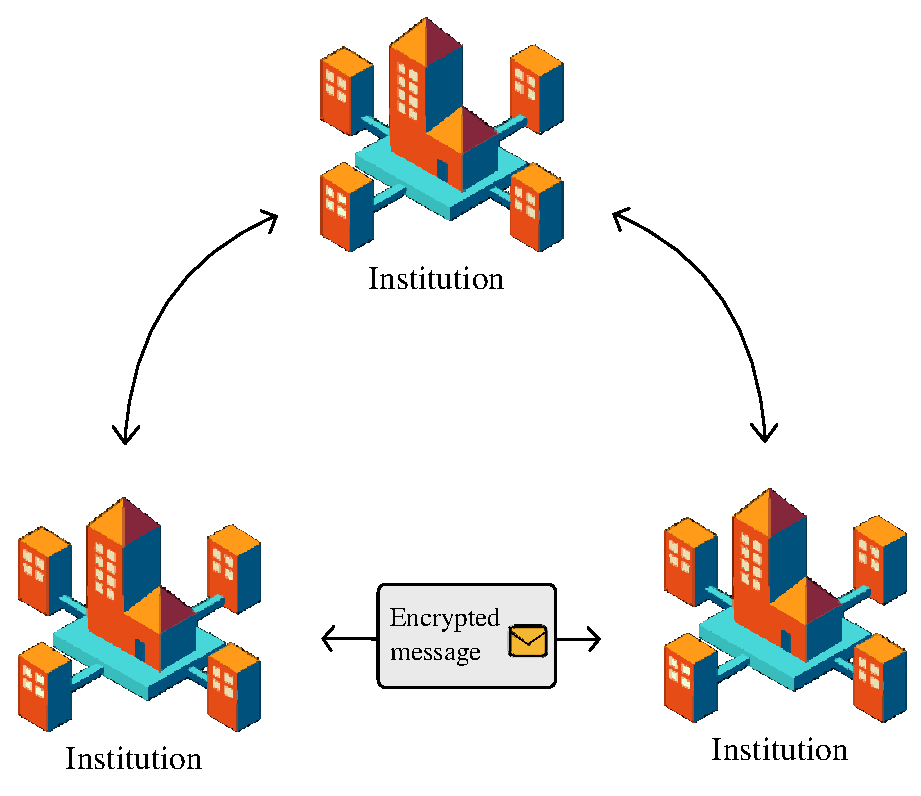
\includegraphics[width=2.5in]{img/fl_sit_ins.eps}%
    \label{fl_sit_institution}}
    \hfil
    \subfloat[Server-based]{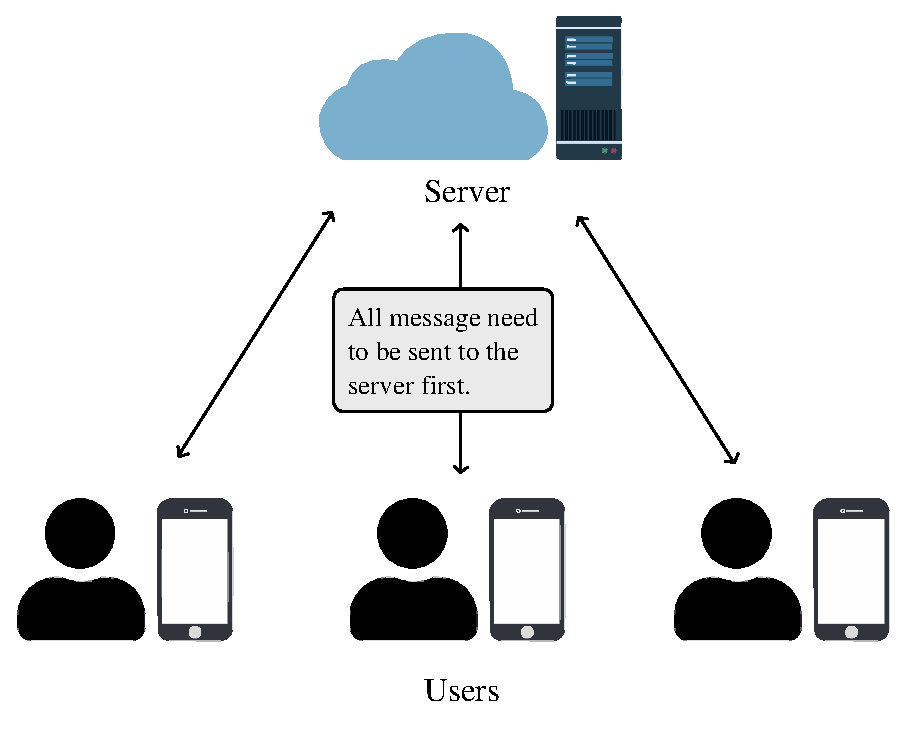
\includegraphics[width=2.5in]{img/fl_sit_server.eps}%
    \label{fl_sit_server}}
    \caption{The structures of two work environments in FL. The first is the ``Among-institutions'' model where institutions can communicate with others directly, and the second is ``Server-based'' model where parties exchange information in virtue of the server.}
    \label{fl_sit}
\end{figure}

\subsection{Multi-party Computation}
Secure MPC is a branch of cryptography which enables several parties to compute a particular function without leaking their own data (inputs). Suppose there are $n$ parties employing MPC to compute a function $F$, and the $i^{th}$ party has its parameter $A_i$. Their goal is to compute $R = F(A_1, A_2, ..., A_n)$. MPC has the feature that participants can only obtain $R$ from the process and the party $P_i$ has no idea about parameter $A_j (j \ne i)$. This feature fits the aggregation algorithm in FL greatly.

Most MPC protocols depend on two cryptography technologies: secret sharing~\cite{Shamir} and oblivious transfer~\cite{OT}. MPC can be implemented with garbled circuits, multi-party circuit-based protocols, or hybrid methods~\cite{mpc-sok}. It also benefits from fully homomorphic encryption (FHE) algorithms. Garbled circuits and FHE suffer from complicated design and poor efficiency. Therefore, secret sharing methods are more favored to solve the privacy-preserving problem in FL. A secret sharing scheme involves a secret $s$, a set of $n$ parties, and a collection $A$ of subsets of parties. Each party has its share of $s$. The secret sharing scheme ensures any subset in $A$ can reconstruct $s$~\cite{Secret-Sharing-survey}. 

SPDZ~\cite{SPDZ} (speedz) is a practical and secure secret-sharing-based MPC protocol introduced by Damgard \emph{et al}. It supports addition and multiplication by means of the triples~\cite{Triple}, which are generated by somewhat homomorphic encryption (SHE). Our method does not require multiplication and hence we do not need to generate the triples. We adopt the resharing method used in SPDZ to achieve secure addition in DemoFL, which is essential in the aggregation phase of FL.


\subsection{Consensus Algorithms}
In a distributed or multi-party system, there is always a problem with consensus, i.e., in such systems parties always need to achieve agreement on a certain value. This could be difficult without any strategy because different parties may be in different statuses and have multifarious matters. Consensus algorithms are adopted to address such problems. It is widely used in blockchain and various famous areas.

Paxos was the first consensus algorithm introduced by Lamport~\cite{Paxos}. It helps the nodes of a cluster to select several leaders democratically and reach a consensus with the help of these leaders. Paxos is used in a lot of famous projects such as Ceph~\cite{Ceph}. Raft is a modification of Paxos which is more implement-friendly~\cite{Raft}. It contains two phases: leader election and log replication. Parties can achieve agreements based on leaders. Considering that FL models are semi-decentralized systems, our framework can utilize Raft algorithm to select several leaders, based on which MPC protocols can be executed efficiently and robustly.